\subsection{Current Solution}
\label{description:solution}
Currently Tomboy has the functionality to create bullet lists in Notes and and with help of the Backlink Addin (which is shipped with the default Tomboy installation) to add Hyperlinks between different Notes. This allows the user to create simple Tasklists through Bulletlist and through linking a single task to another Note to create subtasks. This functionality is also shown in the GUI Mockup in Figure \ref{gui}.

The idea of adding extended task management capability to Tomboy is not new and has been done before already:\\
There is a project (realized as an Addin) for task management, called \textit{Tasks}, created by Boyd Timothy
for quite some time. However, this was removed in Version 0.9.3 of Tomboy, because there were too many problems with the existing implementation\footnote{\url{http://lists.beatniksoftware.com/pipermail/tomboy-list-beatniksoftware.com/2008-January/000540.html}}. Timothy abandoned the code and created a new program called \textit{Tasque}\footnote{\url{http://live.gnome.org/Tasque}} with its main focus just on task management.

In 2009 a new Addin was initiated by Sandy Armstrong. This unfinished project, called \textit{TaskLists}\footnote{\url{http://gitorious.org/~sandy/tomboy/sandys-tomboy/commits/task-lists2}} is still in a very early phase and has not much functionality yet. At the moment nobody is regularly working on it.

That being said, we can conclude that there was a lot of effort done in the past to give Tomboy some more advanced capability of handling task lists than just plain bullet lists, the solution that was created at the beginning was too different from Tomboy to be acceptable. It was a totally separate task management UI in Tomboy that was not integrated in the existing note structure at all. The Tasks Addin added additional GUI elements within Tomboy that made it look more like a separate application besides Tomboy instead of really integrating itself in Tomboy.

Our goal is to finish such a project up to a stable and working solution (in terms of \textit{bug-freeness} and \textit{usability}) that is fully integrated into Tomboys existing concepts and easy and simple to use, such that it could hopefully accepted to be included in the Tomboy project and  shipped with future Tomboy releases.

\subsection{Product Perspective}
\label{description:perspective}
  The project TaskList will be part of the Tomboy project. There will be three main interfaces:

  \begin{itemize}
    \item The first one is the obvious user interface that the user sees within Tomboy.
    \item Then, the representation of data will be done via Tomboy note files. That means, persistent storage of the Tasks must be accomplished as xml files within the Tomboy notes file structure.
    \item Also, saving and retrieving data (for example, import and export of notes from/to other note taking applications) will be done using XML files.
  \end{itemize}

  Also, for an overwie of the integration of TaskList within the Tomboy/GTK/Mono context, see figure \ref{perspective}.

  \begin{figure}[h]
    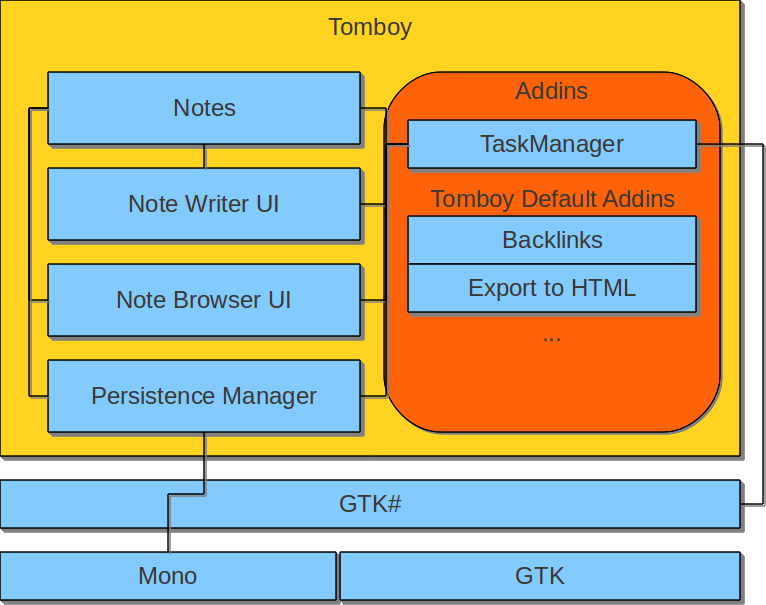
\includegraphics[width=\textwidth]{graphics/product_perspective_diagram.png}
    \caption{TaskList Product Perspective}
    \label{perspective}
  \end{figure}


\subsection{Product Functions}
\label{description:functions}

  \subsubsection*{Supported Functions}
  \label{description:functions:supported}

    \begin{itemize}
      \item Provides Task management capabilities for Tomboy
      \item Supports multiple Tasks and TaskLists as well as Subtasks
      \item Supports priorities and due dates
      \item Allows to create dependencies between tasks
      \item Allows easy management of TaskLists and Tasks
      \item Allows to import export TaskLists
    \end{itemize}

    \subsubsection*{Unsupported Functions}
      \label{description:functions:unsupported}
      \begin{itemize}
        \item Does not have additional GUI windows or external tools within or outside of Tomboy. (SEE ?) %TODO reference
        \item Does not support synchronisation with external tools or clients except for manual export / import.
      \end{itemize}

\subsection{User Characteristics}
\label{description:usercharacteristics}

  \begin{itemize}
    \item[Casual user] The casual user will create simple task lists. He may or may not know very vell the functionality of Tomboy. Still, he should be able to create simple TaskLists where he can cross out individual elements easily.

    \item [Advanced user] The advanced user knows and uses Tomboy already quite well. He should be able without too much effort to add arguments such as due dates and priorities to his task lists, create hierarichies of tasks and may his lists to other tools, e.g. \textit{Evolution}.
  \end{itemize}


\subsection{Constraints}
\label{description:constraints}
The Addin itself should obey all criterias (standards and guidelines) imposed by the GNOME and Tomboy projects (SEE ?). %TODO

Besides the coding guidelines this includes mainly design aspects, such as simplicity and easyness of use, and full integration into Tomboy (see also \ref{?}).


\subsection{Assumptions and Dependencies}
\label{description:assumptions}

